\documentclass[aspectratio=169]{beamer}
\usepackage{graphicx}
\usepackage{amsmath}
\usepackage{amssymb}
\usepackage{booktabs} % For nice tables
\usepackage{tikz}
\usetikzlibrary{arrows.meta,positioning,fit,shapes,calc}

% --- Beamer Theme & Info ---
\usetheme{Rochester}
\usecolortheme{default}
\setbeamertemplate{navigation symbols}{}
\setbeamertemplate{footline}[frame number]

\title{Probabilistic Model}
\author{Chanon Puttanawarut}

% --- Section divider slides (generated automatically for every \section) ---
\AtBeginSection[]{
  \begin{frame}
    \vfill
    \centering
    {\usebeamerfont{title}\usebeamercolor[fg]{structure}\insertsectionhead\par}
    \vfill
  \end{frame}
}

% --- TikZ styles (shared by all figures) ---
\tikzset{
  class/.style={circle, draw=blue!60, fill=blue!5, very thick, minimum size=10mm, font=\small},
  feature/.style={circle, draw=red!60, fill=red!5, very thick, minimum size=10mm, font=\small},
  box/.style={rectangle, rounded corners=3pt, draw=blue!60, fill=blue!5, very thick,
              minimum height=7mm, inner sep=4pt, font=\small, align=center},
  mynode/.style={circle, draw=blue!60, fill=blue!5, very thick, minimum size=8mm},
  latent/.style={circle, draw=black!70, fill=white, thick, minimum size=10mm},
  obs/.style={circle, draw=black!70, fill=black!15, thick, minimum size=10mm},
  param/.style={circle, draw=black!70, fill=white, thick, minimum size=7mm, inner sep=1pt},
  plate/.style={draw, rounded corners=2pt},
  edge/.style={->, thick}
}

\begin{document}

% --- Title Slide ---
\begin{frame}
  \titlepage
\end{frame}

% --- Outline Slide ---
\begin{frame}{Outline}
  \tableofcontents
\end{frame}

%%%%%%%%%%%%%%%%%%%%%%%%%%%%%%%%%%%%%%%%%%%%%%%%%%%%
\section{Learning from Data: MLE}
%%%%%%%%%%%%%%%%%%%%%%%%%%%%%%%%%%%%%%%%%%%%%%%%%%%%

\begin{frame}{Learning}
\begin{itemize}
  \item Data are generated by a process (a ``machine'') with parameters $\theta$.
  \item We choose the \emph{form} of $p(\text{Data}\mid\theta)$ (e.g.\ Bernoulli, Normal), but we do not know $\theta$.
  \item Goal: infer $\theta$ from observed data.
\end{itemize}
\[
  \text{Given data } X,\ \text{find } \hat{\theta}
\]
\end{frame}

\begin{frame}{Probability Basics (Quick Recap)}
\begin{itemize}
  \item Conditional probability: $p(X\mid Y) = \dfrac{p(X,Y)}{p(Y)}$
  \item Product rule: $p(X,Y) = p(X\mid Y)\,p(Y)$
  \item Bayes' theorem: $p(Y\mid X) = \dfrac{p(X\mid Y)\,p(Y)}{p(X)}$
  \item Independence: $X \perp Y \iff p(X,Y) = p(X)\,p(Y)$
  \item Expectation: $\mathbb{E}[X] = \sum_x x\, p(x)$ or $\int x\, p(x)\,dx$
  \item Common distributions: Bernoulli, Categorical, Multinomial, Normal
\end{itemize}
\end{frame}

\begin{frame}{Maximum Likelihood Estimation (MLE)}
\begin{block}{Maximum Likelihood Estimation}
\[
  \hat{\theta} = \arg\max_{\theta}\; p(X\mid\theta)
\]
\end{block}
\begin{itemize}
  \item Choose the $\theta$ that makes the observed data most probable.
  \item If the data points $x_1,\dots,x_N$ are i.i.d.:
  \[
    p(X\mid\theta) = \prod_{n=1}^{N} p(x_n\mid\theta)
    \qquad\Rightarrow\qquad
    \log p(X\mid\theta) = \sum_{n=1}^{N} \log p(x_n\mid\theta)
  \]
  \item Maximizing the log-likelihood gives the same $\hat\theta$ ($\log$ is increasing) and is easier to work with.
  \item Many machine learning loss functions (e.g.\ cross-entropy, squared error) are negative log-likelihoods.
\end{itemize}
\end{frame}

\begin{frame}{Example: Coin Flipping}
Two candidate models:
\begin{align*}
  \text{Straight coin: } & p(H)=\tfrac{1}{2},\quad p(T)=\tfrac{1}{2} \\
  \text{Bent coin: }     & p(H)=\tfrac{4}{5},\quad p(T)=\tfrac{1}{5}
\end{align*}
Observed data $D$: HTHHHTHHTHTH \quad (8 heads, 4 tails)

\vspace{0.4cm}
Which model makes $D$ more probable? \;Compare $p(D\mid\text{Straight})$ with $p(D\mid\text{Bent})$.
\end{frame}

\begin{frame}{Coin Flip: Computing Likelihoods}
Observed data $D$: HTHHHTHHTHTH (8 heads, 4 tails)
\begin{align*}
  p(D\mid\text{Straight}) &= \left(\tfrac{1}{2}\right)^{12} \approx 2.44\times 10^{-4} \\
  p(D\mid\text{Bent})     &= \left(\tfrac{4}{5}\right)^{8}\left(\tfrac{1}{5}\right)^{4} \approx 2.68\times 10^{-4}
\end{align*}
\[
  \frac{p(D\mid\text{Bent})}{p(D\mid\text{Straight})} \approx 1.10
  \quad\Rightarrow\quad \text{MLE chooses the bent coin}
\]
\begin{alertblock}{Careful with the wording}
The \emph{data} are about 1.1 times more probable under the bent coin.
This compares $p(D\mid\text{coin})$, \textbf{not} $p(\text{coin}\mid D)$:
it does not say that the bent coin is more likely to be the coin we are holding.
\end{alertblock}
\end{frame}

\begin{frame}{MLE for a Bernoulli Parameter}
\begin{columns}[c]
\column{0.5\textwidth}
Let $\theta = p(H)$ be \emph{any} value in $[0,1]$.\\
With 8 heads and 4 tails, $L(\theta) = \theta^{8}(1-\theta)^{4}$:
\[
  \log L(\theta) = 8\log\theta + 4\log(1-\theta)
\]
Set the derivative to zero:
\[
  \frac{8}{\theta} - \frac{4}{1-\theta} = 0
  \;\Rightarrow\;
  \hat\theta = \frac{8}{12} \approx 0.67
\]
\textbf{In general:} \ $\hat\theta = \dfrac{\#\text{heads}}{N}$ \ (count / total).

\vspace{0.2cm}
Naive Bayes estimates its parameters exactly like this.
\column{0.5\textwidth}
\centering
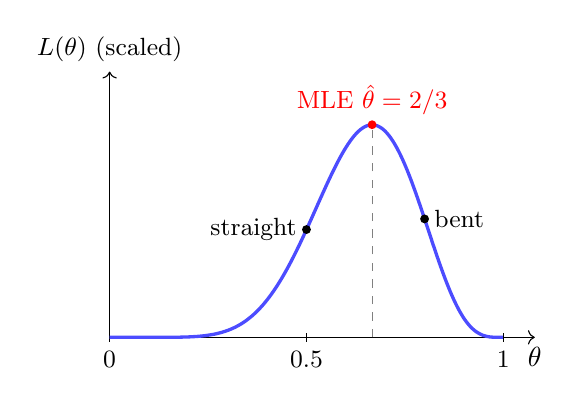
\begin{tikzpicture}[x=5cm, y=2.7cm]
  \draw[->] (0,0) -- (1.08,0) node[below] {$\theta$};
  \draw[->] (0,0) -- (0,1.25) node[above] {\small $L(\theta)$ (scaled)};
  \foreach \t in {0,0.5,1} \draw (\t,0.02) -- (\t,-0.02) node[below] {\small $\t$};
  \draw[very thick, blue!70, domain=0:1, samples=120, smooth]
    plot (\x, {(1.5*\x)^8 * (3*(1-\x))^4});
  \draw[dashed, gray] (2/3,0) -- (2/3,1);
  \fill[red] (2/3,1) circle (1.6pt) node[above] {\small MLE $\hat\theta = 2/3$};
  \fill (0.5,0.507) circle (1.6pt) node[left] {\small straight};
  \fill (0.8,0.557) circle (1.6pt) node[right] {\small bent};
\end{tikzpicture}

\small With only two coins to choose from, MLE picks the better of the two (bent).
\end{columns}
\end{frame}

\begin{frame}{Two Problems with MLE}
\begin{enumerate}
  \item \textbf{It ignores prior knowledge.}
  \begin{itemize}
    \item The coin came from a national mint, so it is very probably straight.
    \item MLE still chooses the bent coin, because it only looks at $p(D\mid\theta)$.
  \end{itemize}
  \vspace{0.2cm}
  \item \textbf{It gives extreme answers with little data.}
  \begin{itemize}
    \item Flip a coin 3 times: HHH. \quad MLE: $\hat\theta = 3/3 = 1$.
    \item So the next flip is heads with probability 1, and tails is \emph{impossible}?
  \end{itemize}
\end{enumerate}
\vspace{0.3cm}
\begin{block}{Plan}
Problem 1 $\to$ use Bayes' rule with a prior (next section).\\
Problem 2 $\to$ smoothing (we will meet it again in Naive Bayes).
\end{block}
\end{frame}

%%%%%%%%%%%%%%%%%%%%%%%%%%%%%%%%%%%%%%%%%%%%%%%%%%%%
\section{Bayes' Rule for Decisions}
%%%%%%%%%%%%%%%%%%%%%%%%%%%%%%%%%%%%%%%%%%%%%%%%%%%%

\begin{frame}{Bayes' Rule: Prior, Likelihood, Posterior}
Let $h$ be a hypothesis (which coin? which class?) and $D$ the observed data.
\begin{block}{Bayes' rule}
\[
  \underbrace{p(h\mid D)}_{\text{posterior}}
  = \frac{\overbrace{p(D\mid h)}^{\text{likelihood}}\ \overbrace{p(h)}^{\text{prior}}}{\underbrace{p(D)}_{\text{evidence}}},
  \qquad
  p(D) = \sum_{h'} p(D\mid h')\,p(h')
\]
\end{block}
\begin{itemize}
  \item \textbf{Prior} $p(h)$: what we believe before seeing the data.
  \item \textbf{Likelihood} $p(D\mid h)$: how well $h$ explains the data.
  \item \textbf{Posterior} $p(h\mid D)$: what we believe after seeing the data.
  \item \textbf{Evidence} $p(D)$: the same for every $h$, so $p(h\mid D) \propto p(D\mid h)\,p(h)$.
\end{itemize}
\end{frame}

\begin{frame}{Back to the Coin: Adding a Prior}
\textbf{Two hypotheses:}
\begin{align*}
  h_1 &: \text{straight coin}, \quad p(H)=\tfrac{1}{2} \\
  h_2 &: \text{bent coin}, \quad p(H)=\tfrac{4}{5}
\end{align*}
\textbf{Prior} (the coin came from a mint, so it is probably straight):
\[
  p(h_1) = 0.9, \qquad p(h_2) = 0.1
\]
\textbf{Data:} HTHHHTHHTHTH (8 heads, 4 tails)

\vspace{0.3cm}
\textbf{Question:} after seeing the flips, how probable is each coin?
\end{frame}

\begin{frame}{Computing the Posterior}
\centering
\small
\begin{tabular}{lcccc}
\toprule
 & Prior $p(h)$ & Likelihood $p(D\mid h)$ & $p(D\mid h)\,p(h)$ & Posterior $p(h\mid D)$ \\
\midrule
Straight $h_1$ & 0.9 & $2.44\times10^{-4}$ & $2.197\times10^{-4}$ & \textbf{0.891} \\
Bent $h_2$     & 0.1 & $2.68\times10^{-4}$ & $0.268\times10^{-4}$ & \textbf{0.109} \\
\midrule
Sum            & 1   &                     & $p(D) = 2.466\times10^{-4}$ & 1 \\
\bottomrule
\end{tabular}

\vspace{0.4cm}
\normalsize
\raggedright
\begin{enumerate}
  \item Likelihoods: computed before.
  \item Multiply each likelihood by its prior.
  \item Add them up to get the evidence $p(D)$.
  \item Divide by $p(D)$: \quad
  $p(h_1\mid D) = \dfrac{2.197\times10^{-4}}{2.466\times10^{-4}} \approx 0.891$
\end{enumerate}
\end{frame}

\begin{frame}{How Much Does the Prior Matter?}
\centering
\begin{tabular}{lccc}
\toprule
Prior $p(h_1),\ p(h_2)$ & Posterior straight & Posterior bent & Decision \\
\midrule
0.5, 0.5 \ (no preference) & 0.476 & 0.524 & bent \\
0.9, 0.1 \ (from a mint)   & 0.891 & 0.109 & straight \\
\bottomrule
\end{tabular}

\vspace{0.4cm}
\raggedright
\begin{itemize}
  \item With a uniform prior, $p(h\mid D) \propto p(D\mid h)$, so the decision is the same as MLE.
  \item The data favour the bent coin only by a factor of 1.1 (weak evidence), so a strong prior wins.
  \item With many more flips, the likelihood dominates and the prior matters less.
\end{itemize}
\end{frame}

\begin{frame}{From Choosing a Coin to Classifying}
Choosing a coin \emph{is} a classification problem: the class is the coin.

\vspace{0.3cm}
\centering
\begin{tabular}{lll}
\toprule
 & Coin example & Classification \\
\midrule
Hypothesis / class & which coin $h$ & class $Y$ (e.g.\ disease or not) \\
Prior & $p(h)$ & $p(Y)$ \\
Likelihood & $p(\text{flips}\mid h)$ & $p(X_1,\dots,X_n\mid Y)$ \\
Posterior & $p(h\mid\text{flips})$ & $p(Y\mid X_1,\dots,X_n)$ \\
\bottomrule
\end{tabular}

\vspace{0.4cm}
\raggedright
\begin{itemize}
  \item \textbf{Naive Bayes} = this recipe, with a simple way to model $p(X_1,\dots,X_n\mid Y)$.
  \item ``Bayes'' refers to using Bayes' rule over the \emph{class}. The model's parameters are still estimated by MLE (counting), as in Section~1.
\end{itemize}
\end{frame}

%%%%%%%%%%%%%%%%%%%%%%%%%%%%%%%%%%%%%%%%%%%%%%%%%%%%
\section{Naive Bayes}
%%%%%%%%%%%%%%%%%%%%%%%%%%%%%%%%%%%%%%%%%%%%%%%%%%%%

\begin{frame}{Naive Bayes}
\begin{itemize}
  \item A \textbf{generative classifier}: it models how the data are generated, through $p(Y)$ and $p(X\mid Y)$.
  \item To predict, apply Bayes' rule:
  \[
    p(Y=y\mid X=x)=\frac{p(X=x\mid Y=y)\,p(Y=y)}{\sum_{y'} p(X=x\mid Y=y')\,p(Y=y')}
  \]
  \item The denominator is the same for every $y$, so for the decision we only need
  \[
    \hat y = \arg\max_{y}\; p(Y=y)\,p(X=x\mid Y=y)
  \]
  \item It is called \textbf{naive} because it assumes that the features are conditionally independent given the class (next slides).
\end{itemize}
\end{frame}

\begin{frame}{Conditional Independence}
\begin{columns}[c]
\column{0.68\textwidth}
\begin{block}{Definition: $A \perp B \mid C$ \ (conditionally independent given $C$)}
$p(A,B\mid C) = p(A\mid C)\,p(B\mid C)$,\\[2pt]
or equivalently \ $p(A\mid B,C) = p(A\mid C)$
\end{block}
\textbf{Example:} fever and cough
\begin{itemize}
  \item Overall they are \emph{dependent}: both are caused by the disease.
  \item Assumption: \emph{once we know the disease status}, fever tells us nothing more about cough.
\end{itemize}
Note: independence and conditional independence are different; neither implies the other.
\column{0.28\textwidth}
\centering
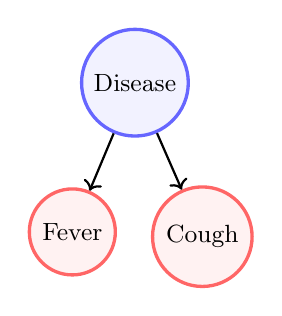
\begin{tikzpicture}
  \node[class] (Y) {Disease};
  \node[feature, below left=1.0cm and -0.1cm of Y] (A) {Fever};
  \node[feature, below right=1.0cm and -0.1cm of Y] (B) {Cough};
  \draw[edge] (Y) -- (A);
  \draw[edge] (Y) -- (B);
\end{tikzpicture}
\end{columns}
\end{frame}

\begin{frame}{The Naive Bayes Assumption}
\begin{block}{Features are conditionally independent given the class}
\[
  p(X_1,\dots,X_n\mid Y)=\prod_{i=1}^n p(X_i\mid Y)
  \qquad\Rightarrow\qquad
  \hat y = \arg\max_y\; p(y)\prod_{i=1}^n p(x_i\mid y)
\]
\end{block}
\textbf{Why it helps:} number of parameters for $n$ binary features, per class
\begin{center}
\begin{tabular}{lccc}
\toprule
 & general $n$ & $n=3$ & $n=30$ \\
\midrule
Full joint $p(X_1,\dots,X_n\mid Y)$ & $2^n-1$ & 7 & $\approx 1.07\times 10^{9}$ \\
Naive Bayes $\prod_i p(X_i\mid Y)$  & $n$     & 3 & 30 \\
\bottomrule
\end{tabular}
\end{center}
\begin{itemize}
  \item Each $p(X_i\mid Y)$ is estimated separately, just by counting.
  \item The assumption is usually \emph{not} exactly true, which is why the method is called ``naive''. It still works well in practice.
\end{itemize}
\end{frame}

\begin{frame}{Example: Problem Setup}
\begin{itemize}
  \item Goal: predict whether a patient has the disease ($Y=1$) or not ($Y=0$) from three binary features:
  \begin{itemize}
    \item $X_1$: Fever (1 = yes, 0 = no)
    \item $X_2$: Cough (1 = yes, 0 = no)
    \item $X_3$: Fatigue (1 = yes, 0 = no)
  \end{itemize}
  \item Model: $X_i\mid Y=c \sim \mathrm{Bernoulli}(\theta_{i|c})$, where $\theta_{i|c} = p(X_i=1\mid Y=c)$.
  \item Small training set of $N=12$ patients (counts on the next slide).
\end{itemize}
\end{frame}

\begin{frame}{Example: Training Counts (Toy Dataset)}
\centering
\begin{tabular}{l c c}
\toprule
 & Disease ($Y=1$) & No disease ($Y=0$) \\
\midrule
Number of patients & $N_{1}=5$ & $N_{0}=7$ \\
Fever ($X_1=1$)    & 4 & 2 \\
Cough ($X_2=1$)    & 3 & 5 \\
Fatigue ($X_3=1$)  & 5 & 2 \\
\bottomrule
\end{tabular}

\vspace{10pt}
Class prior (MLE, count / total): \quad
\(\hat p(Y=1)=\dfrac{5}{12},\quad \hat p(Y=0)=\dfrac{7}{12}\)
\end{frame}

\begin{frame}{Example: Estimate the Class-Conditionals (MLE)}
Same as the coin: each $\theta_{i|c}$ is a Bernoulli parameter, so its MLE is count / total:
\[
  \hat\theta_{i|c} = \hat p(X_i=1\mid Y=c)=\frac{\text{count}(X_i=1,\ Y=c)}{N_c}
\]
\centering
\begin{tabular}{lcc}
\toprule
 & $Y=1$ & $Y=0$ \\
\midrule
$\hat p(X_1=1\mid Y)$ \ (Fever)   & $4/5 = 0.80$ & $2/7 \approx 0.286$ \\
$\hat p(X_2=1\mid Y)$ \ (Cough)   & $3/5 = 0.60$ & $5/7 \approx 0.714$ \\
$\hat p(X_3=1\mid Y)$ \ (Fatigue) & $5/5 = 1.00$ & $2/7 \approx 0.286$ \\
\bottomrule
\end{tabular}
\end{frame}

\begin{frame}{Example: Classify a New Patient}
New patient: Fever = 1, Cough = 0, Fatigue = 1, \ i.e.\ $x=(1,0,1)$.
\[
  s_c = \hat p(Y=c)\prod_{i=1}^3 \hat p(X_i=x_i\mid Y=c),
  \qquad \hat p(X_i=0\mid Y=c) = 1-\hat\theta_{i|c}
\]
\begin{align*}
  s_{1} &= \tfrac{5}{12}\times 0.80\times (1-0.60)\times 1.00 \approx 0.1333\\
  s_{0} &= \tfrac{7}{12}\times 0.286\times (1-0.714)\times 0.286 \approx 0.0136
\end{align*}
Normalize (divide by the sum, which is $\hat p(x)$):
\[
  p(Y=1\mid x) \approx\frac{0.1333}{0.1333+0.0136} \approx 0.907,\qquad
  p(Y=0\mid x) \approx 0.093
\]
Prediction: \textbf{disease}.
\end{frame}

\begin{frame}{Problem: Zero Probabilities}
All 5 disease patients had fatigue, so MLE gives
\[
  \hat p(X_3=1\mid Y=1) = \tfrac{5}{5} = 1
  \quad\Rightarrow\quad
  \hat p(X_3=0\mid Y=1) = 0
\]
Another new patient: Fever = 1, Cough = 1, Fatigue = 0, \ i.e.\ $x=(1,1,0)$:
\begin{align*}
  s_1 &= \tfrac{5}{12}\times 0.80 \times 0.60 \times \mathbf{0} = 0\\
  s_0 &= \tfrac{7}{12}\times 0.286 \times 0.714 \times 0.714 \approx 0.0850
\end{align*}
\begin{alertblock}{One unseen value vetoes the whole product}
$p(Y=1\mid x) = 0$, whatever the other features say.\\
This is the HHH problem again: 5 out of 5 is not enough evidence to conclude ``always''.
\end{alertblock}
\end{frame}

\begin{frame}{Laplace (Add-$\alpha$) Smoothing}
Pretend that we saw $\alpha$ extra examples of \emph{each} possible value (pseudo-counts):
\[
  \hat p_{\alpha}(X_i=k\mid Y=c) = \frac{\text{count}(X_i=k,\ Y=c)+\alpha}{N_c+\alpha K}
\]
where $K$ is the number of values that $X_i$ can take ($K=2$ for binary features).
$\alpha=1$ is called \emph{Laplace smoothing}.

\vspace{0.3cm}
\begin{itemize}
  \item Coin with HHH: \ $\hat p(H) = \dfrac{3+1}{3+2} = 0.8$ \ instead of $1$.
  \item Fatigue: \ $\hat p(X_3=0\mid Y=1) = \dfrac{0+1}{5+2} = \dfrac17 \approx 0.143$ \ instead of $0$.
  \item The pseudo-counts act like a prior belief that every value is possible. As $N_c$ grows, their effect disappears.
\end{itemize}
\end{frame}

\begin{frame}{Example with Laplace Smoothing ($\alpha=1$, $K=2$)}
\centering
\begin{tabular}{lcc}
\toprule
 & $Y=1$ & $Y=0$ \\
\midrule
$\hat p(X_1=1\mid Y)$ \ (Fever)   & $(4+1)/(5+2) = 5/7$ & $(2+1)/(7+2) = 3/9$ \\
$\hat p(X_2=1\mid Y)$ \ (Cough)   & $(3+1)/(5+2) = 4/7$ & $(5+1)/(7+2) = 6/9$ \\
$\hat p(X_3=1\mid Y)$ \ (Fatigue) & $(5+1)/(5+2) = 6/7$ & $(2+1)/(7+2) = 3/9$ \\
\bottomrule
\end{tabular}

\vspace{0.4cm}
\begin{tabular}{lcc}
\toprule
New patient & $p(Y=1\mid x)$ without smoothing & $p(Y=1\mid x)$ with smoothing \\
\midrule
$x=(1,1,0)$ & 0     & 0.219 \\
$x=(1,0,1)$ & 0.907 & 0.835 \\
\bottomrule
\end{tabular}

\vspace{0.4cm}
\raggedright
Smoothing removes the hard zero and makes the model less over-confident.
(The class priors stay at $5/12$ and $7/12$.)
\end{frame}

\begin{frame}{In Practice: Work in Log Space}
\begin{itemize}
  \item A product of many probabilities becomes too small for the computer.\\
  Example: a document with 500 words, each with probability $\approx 10^{-3}$, gives $10^{-1500}$,
  but a 64-bit float stops at about $10^{-308}$, so every class gets a score of $0$.
  \item Take logs: the product becomes a sum, and the $\arg\max$ does not change because $\log$ is increasing:
  \[
    \hat y = \arg\max_c \Big[\log \hat p(Y=c) + \sum_{i=1}^n \log \hat p(X_i=x_i\mid Y=c)\Big]
  \]
  \item Smoothing matters here too: $\log 0 = -\infty$.
  \item Libraries such as scikit-learn do this internally.
\end{itemize}
\end{frame}

\begin{frame}{Naive Bayes Variants: Discrete Features}
Choose the distribution of each feature (given the class) to match the type of data.
\begin{itemize}
  \item \textbf{Bernoulli Naive Bayes} (our disease example)
  \begin{itemize}
    \item Binary features $X_i\in\{0,1\}$.
    \item Model: $X_i\mid Y=c \sim \mathrm{Bernoulli}(\theta_{i|c})$.
    \item Estimate: $\hat\theta_{i|c}=\dfrac{\text{count}(X_i=1,\ Y=c)+\alpha}{N_c+2\alpha}$.
  \end{itemize}
  \item \textbf{Categorical Naive Bayes}
  \begin{itemize}
    \item Features with $K_i$ unordered values, e.g.\ colour $\in\{\text{red},\text{green},\text{blue}\}$.
    \item Model: $X_i\mid Y=c \sim \mathrm{Categorical}(\theta_{i,1|c},\dots,\theta_{i,K_i|c})$, \
          i.e.\ $p(X_i=k\mid Y=c)=\theta_{i,k|c}$, \ $\sum_{k}\theta_{i,k|c}=1$.
    \item Estimate: $\hat\theta_{i,k|c}=\dfrac{\text{count}(X_i=k,\ Y=c)+\alpha}{N_c+\alpha K_i}$.
  \end{itemize}
\end{itemize}
\end{frame}

\begin{frame}{Naive Bayes Variants: Gaussian Naive Bayes}
\begin{itemize}
  \item For continuous features $X_i\in\mathbb{R}$ (measurements, sensor data).
  \item Model: $X_i\mid Y=c \sim \mathcal{N}(\mu_{i|c},\,\sigma^2_{i|c})$, with density
  \[
    p(x_i\mid Y=c) = \frac{1}{\sqrt{2\pi\sigma^2_{i|c}}} \exp\!\left(-\frac{(x_i-\mu_{i|c})^2}{2\sigma^2_{i|c}}\right)
  \]
  \item MLE from the $N_c$ training examples of class $c$:
  \[
    \hat{\mu}_{i|c} = \frac{1}{N_c}\sum_{n:\,y_n=c} x_{n,i}, \qquad
    \hat{\sigma}^2_{i|c} = \frac{1}{N_c}\sum_{n:\,y_n=c} (x_{n,i} - \hat{\mu}_{i|c})^2
  \]
  \item $p(x_i\mid Y=c)$ is a \emph{density}, not a probability (it can be larger than 1).
        Bayes' rule still works, because we only compare and normalize across classes.
\end{itemize}
\end{frame}

\begin{frame}{Example: Gaussian Naive Bayes}
Predict flu ($Y=1$) from temperature $X_1$ ($^\circ$C) and heart rate $X_2$ (beats/min).
Parameters estimated from training data:
\begin{center}
\begin{tabular}{lccc}
\toprule
 & Prior & $X_1$: temperature & $X_2$: heart rate \\
\midrule
Flu ($Y=1$)    & 0.3 & $\mu=38.5,\ \sigma=0.5$ & $\mu=95,\ \sigma=10$ \\
No flu ($Y=0$) & 0.7 & $\mu=37.0,\ \sigma=0.5$ & $\mu=75,\ \sigma=10$ \\
\bottomrule
\end{tabular}
\end{center}
New patient: $x=(38.0,\ 80)$. \ Write $\mathcal{N}(x;\mu,\sigma^2)$ for the Normal density at $x$:
\begin{align*}
  s_1 &= 0.3\times \mathcal{N}(38.0;\,38.5,\,0.5^2)\times\mathcal{N}(80;\,95,\,10^2) = 0.3\times 0.484\times 0.0130 \approx 0.00188\\
  s_0 &= 0.7\times \mathcal{N}(38.0;\,37.0,\,0.5^2)\times\mathcal{N}(80;\,75,\,10^2) = 0.7\times 0.108\times 0.0352 \approx 0.00266
\end{align*}
\[
  p(Y=1\mid x) \approx \frac{0.00188}{0.00188+0.00266} \approx 0.41
\]
Temperature points to flu, but heart rate and the prior point the other way: predict \textbf{no flu}.
\end{frame}

\begin{frame}{Naive Bayes Variants: Multinomial Naive Bayes}
\begin{itemize}
  \item For count features, e.g.\ word counts in a document (``bag of words'').
  \item Vocabulary of $d$ words. A document is $x=(x_1,\dots,x_d)$, where $x_w$ is the number of times word $w$ appears; its length is $L=\sum_w x_w$.
  \item Model: $X\mid Y=c \sim \mathrm{Multinomial}(L;\ \theta_{1|c},\dots,\theta_{d|c})$, where $\theta_{w|c}$ is the probability that a word in a class-$c$ document is $w$.
  \item Estimate with smoothing:
  \[
    \hat\theta_{w|c}=\frac{\text{count}(w,c)+\alpha}{\sum_{w'}\text{count}(w',c)+\alpha d},
  \]
  where $\text{count}(w,c)$ is the total number of times $w$ appears in the class-$c$ training documents.
  \item Score: $s_c = \hat p(Y=c)\prod_{w}\hat\theta_{w|c}^{\,x_w}$. \
        The multinomial coefficient $\frac{L!}{x_1!\cdots x_d!}$ is the same for every class, so it cancels.
\end{itemize}
\end{frame}

\begin{frame}{Example: Multinomial Naive Bayes}
\begin{itemize}
  \item Task: classify short documents into Topic A ($Y=1$) or Topic B ($Y=0$).
  \item Vocabulary: $\{\text{apple},\ \text{banana},\ \text{orange}\}$, \ $d=3$.
  \item Training word counts (summed over all documents of each class):
\end{itemize}
\begin{center}
\begin{tabular}{l c c}
\toprule
Word & Topic A (counts) & Topic B (counts) \\
\midrule
apple  & 4 & 1 \\
banana & 3 & 5 \\
orange & 2 & 2 \\
\midrule
Total words & 9 & 8 \\
\bottomrule
\end{tabular}
\end{center}
\begin{itemize}
  \item Class priors: $\hat p(Y=c) = (\text{number of documents in } c) / (\text{total documents})$.
        For simplicity, assume both topics have the same number of documents, so $\hat p(Y=1)=\hat p(Y=0)=0.5$.
\end{itemize}
\end{frame}

\begin{frame}{Example: Multinomial NB -- Estimates}
\begin{itemize}
  \item Laplace smoothing with $\alpha=1$:
  \[
    \hat\theta_{w|c}=\frac{\text{count}(w,c)+\alpha}{\sum_{w'}\text{count}(w',c)+\alpha d}
  \]
  \item Topic A (denominator $=9+1\cdot 3=12$):
  \[
    \hat\theta_{\text{apple}|1}=\frac{4+1}{12}=\frac{5}{12},\quad
    \hat\theta_{\text{banana}|1}=\frac{3+1}{12}=\frac{4}{12},\quad
    \hat\theta_{\text{orange}|1}=\frac{2+1}{12}=\frac{3}{12}
  \]
  \item Topic B (denominator $=8+1\cdot 3=11$):
  \[
    \hat\theta_{\text{apple}|0}=\frac{1+1}{11}=\frac{2}{11},\quad
    \hat\theta_{\text{banana}|0}=\frac{5+1}{11}=\frac{6}{11},\quad
    \hat\theta_{\text{orange}|0}=\frac{2+1}{11}=\frac{3}{11}
  \]
\end{itemize}
\end{frame}

\begin{frame}{Example: Multinomial NB -- Classify}
\begin{itemize}
  \item New document counts: apple = 1, banana = 0, orange = 2.
  \[
    s_c = \hat p(Y=c)\prod_{w}\hat\theta_{w|c}^{\,x_w}
  \]
  \item Unnormalized scores (priors $=0.5$):
  \[
    s_1 = 0.5\cdot\frac{5}{12}\cdot\left(\frac{3}{12}\right)^2
        = \frac{45}{3456}
        \approx 0.0130,
    \qquad
    s_0 = 0.5\cdot\frac{2}{11}\cdot\left(\frac{3}{11}\right)^2
        = \frac{18}{2662}
        \approx 0.0068
  \]
  \item Normalize: \ $p(Y=1\mid x) \approx \dfrac{0.0130}{0.0130+0.0068} \approx 0.66$
  \item Prediction: \textbf{Topic A} ($Y=1$).
\end{itemize}
\end{frame}

\begin{frame}{Complement Naive Bayes (Optional)}
\begin{itemize}
  \item A variant of Multinomial NB for text with \textbf{many, imbalanced classes} (Rennie et al., 2003).
  \item Problem: a small class has few training words, so its $\hat\theta_{w|c}$ are noisy.
  \item Idea: for each class $c$, estimate the word distribution of its \textbf{complement} (all other classes together), which has much more data:
  \[
    \hat\theta_{w|\neg c}=\frac{\sum_{c'\neq c}\text{count}(w,c')+\alpha}{\sum_{c'\neq c}\sum_{w'}\text{count}(w',c')+\alpha d}
  \]
  \item Predict the class whose complement fits the document \emph{worst}: \
  $\hat y = \arg\min_c \sum_w x_w \log \hat\theta_{w|\neg c}$
  \item With only \textbf{2 classes}, the complement of one class is the other class, so CNB decides exactly like MNB with equal priors. The benefit appears with 3 or more classes.
  \item In scikit-learn: \texttt{ComplementNB}.
\end{itemize}
\end{frame}

\begin{frame}{Naive Bayes: Summary}
\begin{columns}[t]
\column{0.48\textwidth}
\textbf{Strengths}
\begin{itemize}
  \item Training is just counting / averaging: one pass over the data.
  \item Few parameters, so it works with little data and many features (e.g.\ text).
  \item Fast prediction; easy to interpret (one $\hat p(x_i\mid y)$ per feature).
\end{itemize}
\column{0.48\textwidth}
\textbf{Weaknesses}
\begin{itemize}
  \item Conditional independence is rarely true. Correlated features are counted twice, so $p(Y\mid x)$ is often over-confident (close to 0 or 1), even when the predicted class is right.
  \item Needs smoothing for unseen values.
  \item Gaussian NB assumes each feature is Normal within each class.
\end{itemize}
\end{columns}
\end{frame}

\begin{frame}{Generative vs Discriminative Classifiers}
\begin{columns}[t]
\column{0.48\textwidth}
\textbf{Generative} (e.g.\ Naive Bayes)
\begin{itemize}
  \item Models $p(Y)$ and $p(X\mid Y)$, then uses Bayes' rule to get $p(Y\mid X)$.
  \item Can generate new examples $x \sim p(X\mid Y=c)$.
  \item Naive Bayes: closed-form training (counting).
\end{itemize}
\column{0.48\textwidth}
\textbf{Discriminative} (e.g.\ logistic regression)
\begin{itemize}
  \item Models $p(Y\mid X)$ directly; does not model how $X$ is generated.
  \item Training usually needs iterative optimization (e.g.\ gradient descent).
\end{itemize}
\end{columns}
\vspace{0.2cm}

\end{frame}

%%%%%%%%%%%%%%%%%%%%%%%%%%%%%%%%%%%%%%%%%%%%%%%%%%%%
\section{Graphical Models}
%%%%%%%%%%%%%%%%%%%%%%%%%%%%%%%%%%%%%%%%%%%%%%%%%%%%

\begin{frame}{What is a Graphical Model?}
\textbf{Key idea:} use a graph to describe how a joint distribution factorizes.
\begin{itemize}
  \item \textbf{Nodes:} random variables (e.g.\ $Y, X_1, X_2$)
  \item \textbf{Edges:} direct dependencies between variables
  \item \textbf{Missing edges:} (conditional) independence assumptions
\end{itemize}
\vspace{0.2cm}
\textbf{Two main types:}
\begin{itemize}
  \item \textbf{Bayesian network} (directed acyclic graph):
        $p(X_1,\ldots,X_n) = \prod_i p(X_i\mid \text{parents}(X_i))$
  \item \textbf{Markov random field} (undirected graph): a product of factors over groups of connected variables
\end{itemize}
\vspace{0.2cm}
\textbf{Why use them?} A compact representation, independence assumptions that are explicit and easy to read, and efficient algorithms for inference and learning.
\end{frame}

\begin{frame}{Example: Cloudy / Sprinkler / Rain / WetGrass}
\begin{columns}[c]
\column{0.36\textwidth}
\centering
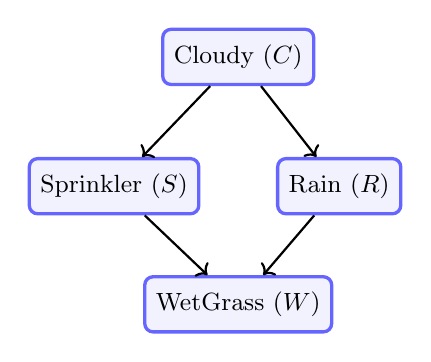
\begin{tikzpicture}
  \node[box] (C) {Cloudy ($C$)};
  \node[box, below left=0.9cm and -0.5cm of C] (S) {Sprinkler ($S$)};
  \node[box, below right=0.9cm and -0.5cm of C] (R) {Rain ($R$)};
  \node[box, below=2.4cm of C] (W) {WetGrass ($W$)};
  \draw[edge] (C) -- (S);
  \draw[edge] (C) -- (R);
  \draw[edge] (S) -- (W);
  \draw[edge] (R) -- (W);
\end{tikzpicture}
\column{0.62\textwidth}
\textbf{Factorization} (one factor per node, given its parents):
\[
  p(C,S,R,W) = p(C)\,p(S\mid C)\,p(R\mid C)\,p(W\mid S,R)
\]
\textbf{Intuition:}
\begin{itemize}
  \item Cloudy weather makes rain more likely, and makes people less likely to turn on the sprinkler.
  \item The grass gets wet from the sprinkler or from the rain.
\end{itemize}
\end{columns}
\end{frame}

\begin{frame}{Reading the Sprinkler Network}
\textbf{Conditional independencies} (from the missing edges):
\begin{itemize}
  \item No edge between $S$ and $R$: \ $S \perp R \mid C$ \
        (once we know the weather, the sprinkler tells us nothing about rain)
  \item No edge $C\to W$: \ $W \perp C \mid S, R$ \
        (clouds affect the grass only through the sprinkler and the rain)
\end{itemize}
\vspace{0.2cm}
\textbf{Compactness} (all variables binary):
\begin{itemize}
  \item Full joint table: $2^4 - 1 = 15$ parameters.
  \item Network: $p(C)$: 1, \ $p(S\mid C)$: 2, \ $p(R\mid C)$: 2, \ $p(W\mid S,R)$: 4 \ $\Rightarrow$ 9 parameters.
\end{itemize}
\vspace{0.2cm}
\begin{alertblock}{Note}
If every pair of variables is connected, the factorization is just the chain rule: no independence is assumed and nothing is saved. The savings come from the \emph{missing} edges.
\end{alertblock}
\end{frame}

\begin{frame}{Reading Independence from the Graph}
\textbf{Key concept: d-separation.}
$A$ and $B$ are conditionally independent given $C$ if every path between them is ``blocked'' by $C$.

\vspace{0.3cm}
\centering
\begin{tabular}{ccc}
% --- Chain ---
\begin{minipage}[t]{0.28\textwidth}
\centering
\textbf{Chain}\\[0.2cm]
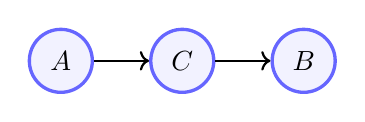
\begin{tikzpicture}[node distance=0.7cm]
\node[mynode] (A) {$A$};
\node[mynode, right=of A] (C) {$C$};
\node[mynode, right=of C] (B) {$B$};
\draw[edge] (A) -- (C);
\draw[edge] (C) -- (B);
\end{tikzpicture}

\vspace{0.1cm}
$A \not\perp B$, \ but $A \perp B \mid C$\\
{\small ($C$ blocks the path)}
\end{minipage}
&
% --- Fork ---
\begin{minipage}[t]{0.28\textwidth}
\centering
\textbf{Fork}\\[0.2cm]
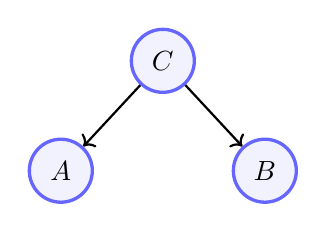
\begin{tikzpicture}
\node[mynode] (C) {$C$};
\node[mynode, below left=0.8cm and 0.7cm of C] (A) {$A$};
\node[mynode, below right=0.8cm and 0.7cm of C] (B) {$B$};
\draw[edge] (C) -- (A);
\draw[edge] (C) -- (B);
\end{tikzpicture}

\vspace{0.1cm}
$A \not\perp B$, \ but $A \perp B \mid C$\\
{\small ($C$ explains both)}
\end{minipage}
&
% --- Collider ---
\begin{minipage}[t]{0.28\textwidth}
\centering
\textbf{Collider}\\[0.2cm]
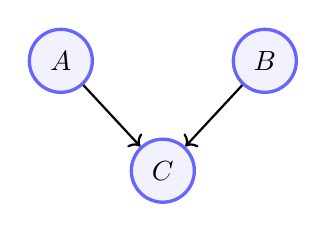
\begin{tikzpicture}
\node[mynode] (C) {$C$};
\node[mynode, above left=0.8cm and 0.7cm of C] (A) {$A$};
\node[mynode, above right=0.8cm and 0.7cm of C] (B) {$B$};
\draw[edge] (A) -- (C);
\draw[edge] (B) -- (C);
\end{tikzpicture}

\vspace{0.1cm}
$A \perp B$, \ but $A \not\perp B \mid C$\\
{\small (observing $C$ connects them)}
\end{minipage}
\end{tabular}

\vspace{0.4cm}
\raggedright
\textbf{Key insight:} the graph structure tells us which conditional independencies hold.
\end{frame}

\begin{frame}{Example: Chain}
\centering
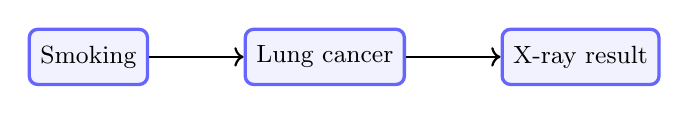
\begin{tikzpicture}[node distance=1.2cm]
  \node[box] (S) {Smoking};
  \node[box, right=of S] (C) {Lung cancer};
  \node[box, right=of C] (X) {X-ray result};
  \draw[edge] (S) -- (C);
  \draw[edge] (C) -- (X);
\end{tikzpicture}

\vspace{0.3cm}
\raggedright
\textbf{Factorization:}
\[
  p(\text{Smoking}, \text{Cancer}, \text{X-ray}) = p(\text{Smoking})\, p(\text{Cancer}\mid\text{Smoking})\, p(\text{X-ray}\mid\text{Cancer})
\]
\textbf{Conditional independence:}
\begin{itemize}
  \item Smoking $\not\perp$ X-ray: they are correlated (through cancer).
  \item But Smoking $\perp$ X-ray $\mid$ Cancer.
  \item Intuition: if we already know the cancer status, the smoking history does not help to predict the X-ray.
\end{itemize}
\end{frame}

\begin{frame}{Example: Fork (Common Cause)}
\centering
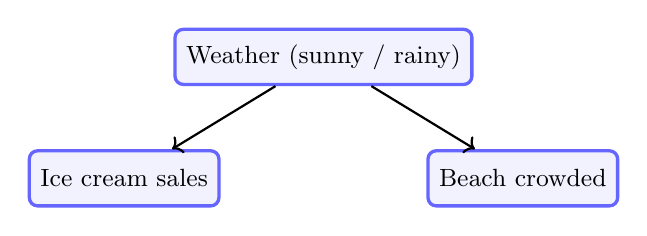
\begin{tikzpicture}
  \node[box] (W) {Weather (sunny / rainy)};
  \node[box, below left=0.8cm and -0.6cm of W] (I) {Ice cream sales};
  \node[box, below right=0.8cm and -0.6cm of W] (B) {Beach crowded};
  \draw[edge] (W) -- (I);
  \draw[edge] (W) -- (B);
\end{tikzpicture}

\vspace{0.2cm}
\raggedright
\textbf{Factorization:}
\[
  p(\text{Weather}, \text{Sales}, \text{Beach}) = p(\text{Weather})\, p(\text{Sales}\mid\text{Weather})\, p(\text{Beach}\mid\text{Weather})
\]
\textbf{Conditional independence:}
\begin{itemize}
  \item Sales $\not\perp$ Beach: they are correlated.
  \item But Sales $\perp$ Beach $\mid$ Weather: the weather explains the correlation.
  \item \textbf{Naive Bayes has exactly this shape:} the class is the common cause of all features.
\end{itemize}
\end{frame}

\begin{frame}{Example: Collider (Common Effect)}
\centering
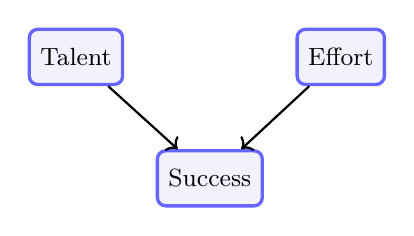
\begin{tikzpicture}
  \node[box] (S) {Success};
  \node[box, above left=0.8cm and 0.4cm of S] (T) {Talent};
  \node[box, above right=0.8cm and 0.4cm of S] (E) {Effort};
  \draw[edge] (T) -- (S);
  \draw[edge] (E) -- (S);
\end{tikzpicture}

\vspace{0.2cm}
\raggedright
\textbf{Factorization:}
\[
  p(\text{Talent}, \text{Effort}, \text{Success}) = p(\text{Talent})\, p(\text{Effort})\, p(\text{Success}\mid\text{Talent}, \text{Effort})
\]
\textbf{Conditional independence:}
\begin{itemize}
  \item Talent $\perp$ Effort (independent in the population).
  \item But Talent $\not\perp$ Effort $\mid$ Success.
  \item \textbf{Explaining away:} among people who succeeded, someone with low talent probably worked hard.
\end{itemize}
\end{frame}

\begin{frame}{Naive Bayes as a Graphical Model}
\begin{columns}[c]
\column{0.42\textwidth}
\centering
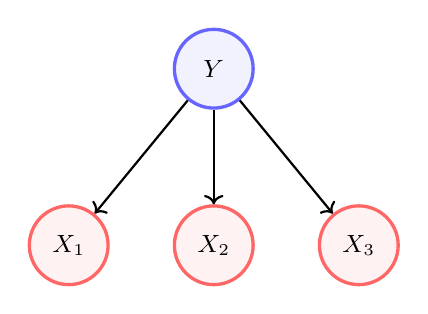
\begin{tikzpicture}
  \node[class] (Y) {$Y$};
  \node[feature, below=1.2cm of Y] (X2) {$X_2$};
  \node[feature, left=0.8cm of X2] (X1) {$X_1$};
  \node[feature, right=0.8cm of X2] (X3) {$X_3$};
  \draw[edge] (Y) -- (X1);
  \draw[edge] (Y) -- (X2);
  \draw[edge] (Y) -- (X3);
\end{tikzpicture}

\vspace{0.2cm}
{\small $Y$ = Disease; \ $X_1$ = Fever,\\ $X_2$ = Cough, $X_3$ = Fatigue}
\column{0.58\textwidth}
\textbf{Factorization:}
\[
  p(Y, X_1, X_2, X_3) = p(Y)\prod_{i=1}^{3} p(X_i\mid Y)
\]
\textbf{Reading the graph:} a \textbf{fork} with $Y$ as the common cause.
\begin{itemize}
  \item $X_i \perp X_j \mid Y$: this is the Naive Bayes assumption.
  \item $X_i \not\perp X_j$ when $Y$ is unknown: the features are still correlated (fever and cough tend to go together).
\end{itemize}
\end{columns}
\end{frame}

\begin{frame}{Plate Notation: Compact Representation of Repetition}
\begin{columns}[c]
\column{0.5\textwidth}
\centering
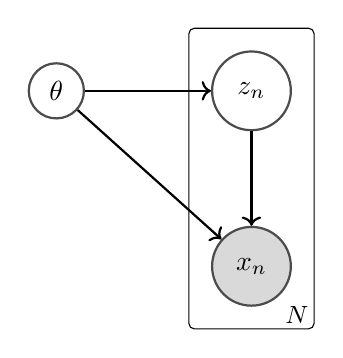
\begin{tikzpicture}
  \node[latent] (z) {$z_n$};
  \node[obs, below=1.2cm of z] (x) {$x_n$};
  \draw[edge] (z) -- (x);
  \node[plate, fit=(z)(x), inner sep=8pt,
        label={[anchor=south east, font=\small, inner sep=2pt]south east:$N$}] (plate) {};
  \node[param, left=1.6cm of z] (theta) {$\theta$};
  \draw[edge] (theta) -- (z);
  \draw[edge] (theta) -- (x);
\end{tikzpicture}
\column{0.5\textwidth}
\begin{itemize}
  \item A \textbf{plate} (box) means: everything inside is repeated; the corner label ($N$) says how many times.
  \item Each data point $n$ has its own $z_n$ and $x_n$.
  \item The parameter $\theta$ is outside the plate: it is shared by all data points.
  \item \textbf{Shaded} nodes are observed; white nodes are not observed.
\end{itemize}
\end{columns}
\end{frame}

\begin{frame}{Naive Bayes with Plate Notation}
\begin{columns}[c]
\column{0.46\textwidth}
\centering
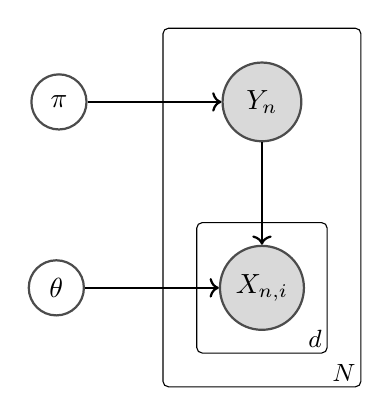
\begin{tikzpicture}
  \node[obs] (Y) {$Y_n$};
  \node[obs, below=1.3cm of Y] (X) {$X_{n,i}$};
  \draw[edge] (Y) -- (X);
  \node[plate, fit=(X), inner sep=8pt,
        label={[anchor=south east, font=\small, inner sep=2pt]south east:$d$}] (pi) {};
  \node[plate, fit=(Y)(pi), inner sep=12pt,
        label={[anchor=south east, font=\small, inner sep=2pt]south east:$N$}] (pn) {};
  \node[param, left=1.7cm of Y] (prior) {$\pi$};
  \node[param, left=1.7cm of X] (theta) {$\theta$};
  \draw[edge] (prior) -- (Y);
  \draw[edge] (theta) -- (X);
\end{tikzpicture}
\column{0.54\textwidth}
\begin{itemize}
  \item Outer plate ($N$): patients. Inner plate ($d$): features of each patient.
  \item $Y_n$ and $X_{n,i}$ are shaded: in training, both are \textbf{observed}.
  \item $\pi$ = class prior, $\theta$ = all $p(X_i\mid Y)$ parameters; outside the plates, so shared by every patient.
  \item The picture encodes the likelihood (maximizing it gives count / total):
  \[
    \prod_{n=1}^{N}\Big[p(y_n\mid\pi)\prod_{i=1}^{d} p(x_{n,i}\mid y_n,\theta)\Big]
  \]
\end{itemize}
\end{columns}
\end{frame}

%%%%%%%%%%%%%%%%%%%%%%%%%%%%%%%%%%%%%%%%%%%%%%%%%%%%
\appendix
%%%%%%%%%%%%%%%%%%%%%%%%%%%%%%%%%%%%%%%%%%%%%%%%%%%%

\begin{frame}{Looking Ahead (Optional): Bayesian Learning}
\begin{itemize}
  \item In this lecture, the parameters $\theta$ were \textbf{fixed numbers} estimated by MLE; Bayes' rule was used only for the class $Y$ (or the coin).
  \item \textbf{Bayesian learning} goes one step further: it treats $\theta$ itself as uncertain, with a prior $p(\theta)$, and applies the same Bayes' rule to it:
  \[
    p(\theta\mid D) \propto p(D\mid\theta)\,p(\theta)
  \]
  \item Example: a coin with a uniform prior on $\theta\in[0,1]$. After HHH, the posterior mean of $\theta$ is $\dfrac{3+1}{3+2}=0.8$, which is exactly Laplace smoothing.
  \item Predictions average over all plausible values of $\theta$:
  \[
    p(x^\ast\mid D)=\int p(x^\ast\mid\theta)\,p(\theta\mid D)\,d\theta
  \]
\end{itemize}
\end{frame}

\end{document}
